\documentclass{article}

\usepackage[dutch]{babel}
\usepackage[margin=3cm]{geometry}
\usepackage{graphicx}
\usepackage{float}
\usepackage{caption}
\usepackage{hyperref}
\usepackage{amsmath}
\usepackage{wrapfig}
\usepackage[parfill]{parskip}

% fonts
\usepackage[T1]{fontenc}
\usepackage{helvet}
\renewcommand{\familydefault}{\sfdefault}

\graphicspath{{img/}}

\newtheorem{theorem}{Definitie}[section]

\usepackage{enumitem}

\newenvironment{thmenum}
 {\begin{enumerate}[label=\upshape\bfseries(\roman*)]}
 {\end{enumerate}}

\usepackage{minted}
\usepackage{upquote}
\usepackage{color}

\begin{document}

\begin{titlepage}
    \author{Tuur Vanhoutte}
    \title{Big Data}
\end{titlepage}

\pagenumbering{gobble}
\maketitle
\newpage
\tableofcontents
\newpage

\pagenumbering{arabic}

\section{Understanding Data Intensive Applications}

\subsection{Why Big Data?}

\subsubsection{Use case: data intensive application RouteYou}

\begin{figure}[H]
    \centering
    \includegraphics[width=0.5\textwidth]{routeyou.png}
    \caption{RouteYou}
\end{figure}

\begin{itemize}
    \item Routes - user preferences \& interests
    \item Searcheable Text data
    \item Geospatial data
    \item Community driven
    \begin{itemize}
        \item Exponential user growth is necessary to make the application posssible
        \item Server power/bills should grow linearly
    \end{itemize}
\end{itemize}

\subsection{Data Intensive Application: RAMS!}

\begin{itemize}
    \item \textbf{Reliable}
    \begin{itemize}
        \item tolerating human mistakes
    \end{itemize}
    \item \textbf{Available}
    \item \textbf{Maintainable}
    \begin{itemize}
        \item Easy to adapt (evolvability)
        \item Easy to deploy \& operate (operations/sys admins)
    \end{itemize}
    \item \textbf{Scalable}
    \begin{itemize}
        \item User growth while maintaining low response times
    \end{itemize}
\end{itemize}

\subsubsection{Common similar abbreviations}

\begin{itemize}
    \item Infrastructure: RAS (Reliable, Available, Serviceable)
    \item Developer: RMS (Reliable, Maintainable, Scalable)
\end{itemize}

\subsubsection{Methods to improve Maintainability}

\begin{itemize}
    \item Github
    \item Error handling
    \item Relative paths (not absolute)
    \item Abstraction (REST API, \dots)
    \item Documentation
\end{itemize}

\subsubsection{RAMS applied to RouteYou application}

\begin{itemize}
    \item Geospatial data (longitude, latitude)
    \item Available \& scalable
    \item Scalable \& low response time
    \item Community driven - unstructured text
    \item Maintainable: automatic classification of community input (ML)
\end{itemize}

\begin{figure}[H]
    \centering
    \includegraphics[width=0.5\textwidth]{RAMS-routeyou.png}
    \caption{To support many users, you need a caching layer}
\end{figure}


\subsection{Learning outcome for this module}

Being able to make infrastructure \& software choices to 
build a Reliable, Available, Maintainable \& Scalable (RAMS) 
data intensive application.

\begin{itemize}
    \item Deep insights into database technology \& cloud services
    \item Connecting with Machine Learning \& AI
    \item Configuring a data back-end (in the cloud or locally)
\end{itemize}


\subsection{Scaling}
\subsubsection{MySQL scaling}

\begin{figure}[H]
    \centering
    \includegraphics[width=0.5\textwidth]{mysql-scaling.png}
    \caption{Transactions/sec }
\end{figure}

\begin{itemize}
    \item Processing power of 16-64 = slightly less then 4x
    \item Real performance: 2.3x
    \item = scaling up: add more processing power to the system
\end{itemize}

\subsubsection{ElasticSearch Scaling: distributed system}

\begin{figure}[H]
    \centering
    \includegraphics[width=0.5\textwidth]{elasticsearch-scaling.png}
    \caption{Response time per request}
\end{figure}

\begin{itemize}
    \item Scaling out: add more servers to your data system
\end{itemize}

\subsubsection{Professional architecture (Dev oriented)}

\begin{figure}[H]
    \centering
    \includegraphics[width=0.5\textwidth]{professional-architecture.png}
    \caption{Professional architecture diagram}
\end{figure}


\begin{itemize}
    \item \textbf{Reverse proxy / Load balancer:} improves scalability
    \item \textbf{Opcode/app/Webserver:} webservice + API
    \item \textbf{Key-value store:} `caching layer'
    \item \textbf{Database server:} distributed storage system + relational database
\end{itemize}

\subsubsection{Time series Distributed database (OpenTSDB, InfluxDB)}

\begin{figure}[H]
    \centering
    \includegraphics[width=0.5\textwidth]{time-series-distributed-db.png}
    \caption{Data from windmill sensors. Most sensors log about every second}
\end{figure}

\begin{itemize}
    \item Losing data is not that big a problem
    \item Massive amount of data to write 
\end{itemize}

\subsection{Scalability \& application performance management}

Response times and percentiles rule the web

\subsubsection{The need for speed: some insights from Google}

\begin{itemize}
    \item Speed is a ranking factor
    \item When your site has high response times, less URLs will be crawled from your site
    \item 53\% of visits are abandoned if a site takes longer than 3 seconds to load
    \item Slow websites will be labeled by Google Chrome
\end{itemize}

\subsubsection{Response times for websites}

\begin{itemize}
    \item \textbf{Ideal:} "blink of an eye" is 300-400 ms
    \item \textbf{Excellent:} 500ms to 1.5 seconds at most
    \item \textbf{Barely acceptable:} 3 seconds
\end{itemize}

Response time = Network latency + processing

\begin{itemize}
    \item 2.9 seconds is faster than 50\% of the web
    \item 1.7 seconds is faster than 75\% of the web
    \item 0.8 seconds is faster than 94\% of the web
\end{itemize}

\subsubsection{4 components of network latency}

\begin{figure}[H]
    \centering
    \includegraphics[width=0.5\textwidth]{network-latency.png}
    \caption{Network latency diagram}
\end{figure}

\begin{itemize}
    \item Processing delay
    \begin{itemize}
        \item Processing network software stack (TCP/IP layers)
        \item Routing decisions
    \end{itemize}
    \item Transmission delay
    \begin{itemize}
        \item Bits on physical link (Bandwidth plays a big role, ex: 1Gbit/s)
    \end{itemize}
    \item Propagation delay
    \begin{itemize}
        \item Speed of EM signals in fiber: 200.000 km/s (67\% of lightspeed)
        \item Changes with distance and medium (Copper: 64\% of lightspeed)
    \end{itemize}
    \item Queing delay
    \begin{itemize}
        \item Time spent in router \& NIC buffers
    \end{itemize}
\end{itemize}

\subsubsection{TCP Congestion Window - slow start}

\begin{itemize}
    \item Network congestion = a network node or link is carrying more data than it can handle
    \item The internet is built around dropped packages
\end{itemize}

\begin{figure}[H]
    \centering
    \includegraphics[width=0.5\textwidth]{tcp-congestion-window.png}
    \caption{TCP Congestion window}
\end{figure}

\begin{itemize}
    \item 4-8-16-32 TCP segments (Win 2008, Win7)
    \item 10-20-40 (Linux 2.6+, Windows Server 2016 / Windows 10)
\end{itemize}

\begin{figure}[H]
    \centering
    \includegraphics[width=0.5\textwidth]{tcp-handshakes.png}
    \caption{Because of many handshakes, there is a lot of latency}
\end{figure}

\begin{itemize}
    \item Solution: KeepAlive of a HTTP Persistent Connection
    \begin{itemize}
        \item Only one 3-way handshake for many requests
        \item Lower network \& CPU load
        \item Lower response times
        \item \textbf{Downside}: more connections open $\Rightarrow$ more memory, more connection failures, app crashing, \dots
    \end{itemize}
\end{itemize}

\begin{itemize}
    \item Measure parallel requests of a website using \url{https://www.webpagetest.org/}
    \item Get a waterfall view of a webpage
\end{itemize}

\subsubsection{Long tail latency}

\begin{figure}[H]
    \centering
    \includegraphics[width=0.5\textwidth]{long-tail-latency.png}
    \caption{Long tail latency vs Normal latency}
\end{figure}


\begin{itemize}
    \item Average = useless
    \item Long tail latency = 99th percentile
    \begin{itemize}
        \item To be experienced by a lot more than 1\% of users!
    \end{itemize}
    \item Best customers encounter highest percentiles
    \item URL consists of many requests
\end{itemize}

\subsection{Conclusion}

\begin{itemize}
    \item Our goal is RAMS (or RASS)
    \item Many data models \& stores: transactional, timeseries, text search
    \item Website 99th percentile + DNS + TCP $\Rightarrow$ < 2s response time
    \begin{itemize}
        \item Efficient caching
        \item Think about your architecture (infrastructure + software) before coding
    \end{itemize}
\end{itemize}

\section{Professional storage}

\subsection{Cloud MIPS}

\begin{figure}[H]
    \centering
    \includegraphics[width=0.5\textwidth]{mips.png}
    \caption{MIPS = Million Instructions Per Second}
\end{figure}

\subsection{Latency vs storage space pyramid}

\begin{figure}[H]
    \centering
    \includegraphics[width=0.7\textwidth]{latency-vs-storage-space-pyramid.png}
    \caption{The higher the performance, the higher the cost per byte of storage}
\end{figure}

\subsection{Storage media}

\subsubsection{Magnetic disks}

\begin{figure}[H]
    \centering
    \includegraphics[width=0.5\textwidth]{magnetic-disks.png}
    \includegraphics[width=0.4\textwidth]{magnetic-disks-performance.png}
    \caption{Massive capacity but mechanical latency}
\end{figure}

\begin{itemize}
    \item Seek time and latency are the key bottlenecks
    \item Need large quantity of disks for good server performance
\end{itemize}

\subsubsection{Flash (NAND) / SSDs}

\begin{figure}[H]
    \centering
    \includegraphics[width=0.5\textwidth]{flash-nand.png}
    \caption{Flash storage}
\end{figure}

\begin{itemize}
    \item SSD = Solid State Drive
    \item NAND = MOSFET + floating gate
    \item Voltage between control gate and N+ : electrons in floating gate
    \item This works very quickly
\end{itemize}

\textbf{Architecture}

\begin{itemize}
    \item Page = 4 KB, pages are in block
    \item Block = 128 pages (4KB * 128 = 512 KB)
    \item You can read or write page per page
    \item Erasing has to erase the entire block
\end{itemize}

\begin{figure}[H]
    \centering
    \includegraphics[width=0.5\textwidth]{flash-architecture.png}
    \caption{Diagram of a flash Block}
\end{figure}


\subsubsection{Big difference between read and writing}

\begin{figure}[H]
    \centering
    \includegraphics[width=0.5\textwidth]{nand-read-write.png}
    \caption{}
\end{figure}

\begin{itemize}
    \item Limited number of writes
    \item Slow block write
    \item Limited "normal" write (programming)
\end{itemize}

\subsubsection{IOPS vs Bandwidth}

\begin{itemize}
    \item Transactions \& virtualized workloads: lots of random access
    \item Timeseries fileserving: mostly sequential
    \item HDD: random performance can be extremely low to medium 
    \item IOPS = Input/Output Operations Per Second
\end{itemize}

\begin{figure}[H]
    \centering
    \includegraphics[width=0.5\textwidth]{storage-device-comparison.png}
    \caption{An enterprise HDD vs an NVME SSD}
\end{figure}

\subsubsection{Storage options}

\begin{figure}[H]
    \centering
    \includegraphics[width=0.6\textwidth]{storage-options.png}
    \caption{Storage options}
\end{figure}

\subsubsection{Performance Conditions}

\begin{figure}[H]
    \centering
    \includegraphics[width=0.6\textwidth]{performance-conditions.png}
    \caption{Performance Conditions}
\end{figure}


\subsection{RAID}

\subsubsection{Definition}

\textbf{Redundant Array of Inexpensive Disks} is a storage technology that combines multiple physical drives into one logical unit.

Purpose:

\begin{itemize}
    \item Data redundancy
    \item Performance improvement
    \item Both
\end{itemize}

\subsubsection{Hardware <> chip}


\subsubsection{Raid levels}

\begin{itemize}
    \item RAID 0
    \item RAID 1
    \item RAID 5
    \item Combinations are possible (RAID 10, 01, 51, 15)
\end{itemize}

\begin{figure}[H]
    \centering
    \includegraphics[width=0.7\textwidth]{raid.png}
    \caption{RAID level choices}
\end{figure}

\subsubsection{Caching \& BBU}

\begin{itemize}
    \item RAM caching: to allow more users to access your data at a time
    \item RAID = lower latency by caching
    \item Not always durable: backup solutions needed like Battery Backup Unit (BBU)
    \item RAID = more bandwitdth, +- same latency
    \begin{itemize}
        \item Latency does not increase as fast when load increases (vs single disk)
        \item More bandwidth \& capacity available
    \end{itemize}
\end{itemize}

\begin{figure}[H]
    \centering
    \includegraphics[width=0.5\textwidth]{raid-caching.png}
    \caption{RAID configuration}
\end{figure}


\subsection{Professional Storage Topology}

\subsubsection{Components}

\begin{itemize}
    \item Enclosure
    \item Controller
    \item Disk Array
    \item HotSpare (=backup disk if a disk fails)
    \item LUN (logical unit number) / Volumes (= logical storage areas)
\end{itemize}

\subsubsection{DAS - Block storage}

\begin{figure}[H]
    \centering
    \includegraphics[width=0.5\textwidth]{das.png}
    \caption{}
\end{figure}

\begin{itemize}
    \item Up to 122 disks per SAS controller
    \item Similar to disks inside the server
    \item No centralized back-up
\end{itemize}


\subsubsection{NAS - File storage}

\begin{figure}[H]
    \centering
    \includegraphics[width=0.5\textwidth]{nas.png}
    \caption{}
\end{figure}

\begin{itemize}
    \item Common Internet File System (CIFS) for Windows
    \item $\rightarrow$ SMB protocol
    \item Network File System (NFS) for UNIX $\Rightarrow$ mounting via network
    \item SMB also available in Linux
\end{itemize}

\subsubsection{SAN - Block storage on a network}

\begin{figure}[H]
    \centering
    \includegraphics[width=0.5\textwidth]{san.png}
    \caption{}
\end{figure}

\begin{itemize}
    \item Seperate Block storage network
    \item Centralized backup \& management
    \item Good scaling, no load on LAN
    \item But:
    \begin{itemize}
        \item No standards - proprietary
        \item Expensive
    \end{itemize}
\end{itemize}

\subsubsection{iSCSI terminology}

\begin{itemize}
    \item iSCSI Target = the iSCSI 'server'
    \begin{itemize}
        \item IP + port = Portal
        \item Portal: LUNs / Volumes
        \item Volume = IQN 
    \end{itemize}
    \item iSCSI Initiator = the iSCSI 'client'
    \begin{itemize}
        \item Connects targets
        \item Find LUNs/Volumes
    \end{itemize}
\end{itemize}

\begin{figure}[H]
    \centering
    \includegraphics[width=0.5\textwidth]{iscsi - layers.jpg}
    \caption{}
\end{figure}

\subsubsection{Object storage}

\begin{itemize}
    \item NAS hardware
    \begin{itemize}
        \item Distributed over multiple datacenters
    \end{itemize}
    \item Object Data
    \begin{itemize}
        \item Metadata
    \end{itemize}
    \item Globally Unique Identifier
    \begin{itemize}
        \item URL
        \item RESTful API
    \end{itemize}
    \item Examples:
    \begin{itemize}
        \item AWS S3
        \item Ceph - Lustre
        \item Google Cloud storage
    \end{itemize}
\end{itemize}

\begin{figure}[H]
    \centering
    \includegraphics[width=0.5\textwidth]{object-storage.png}
    \caption{}
\end{figure}

\subsubsection{Link with Databases \& other data storage}





\begin{itemize}
    \item Transactional database: needs block storage
    \begin{itemize}
        \item Performance
        \item Durability
        \item Consistency
    \end{itemize}
    \item Block storage best for `raw data' (no meta data involved)
    \item NAS = `file based' services like sharepoint
    \item static objects on Object Cloud storage
    \begin{itemize}
        \item good match for OOP \& `unstructured data'
        \item highly available
        \item `Eventually' consistent
    \end{itemize}
\end{itemize}

\section{Relational databases}

Data intensive application: needs RAMS!

\begin{itemize}
    \item \textbf{Reliable}
    \item Available
    \item Maintainable
    \item Scalable
\end{itemize}

\subsection{Components of a relational database}

\begin{itemize}
    \item \textbf{Tables} = Relations are saved in the format of tables
    \item \textbf{Relationships} = a logical connection between different tables
    \begin{itemize}
        \item Join, key, foreign key
        \item Relation schema
    \end{itemize}
    \item \textbf{Tuple} = A single row (record) of a table, which contains a single unordered record for that relation
    \begin{itemize}
        \item A dataset representing an object, an item (`person')
        \item Columns represent the attributes
        \item Tuples are unique
        \item Tuples are similar to Python dictionaries or JavaScript objects
    \end{itemize}
\end{itemize}

\begin{figure}[H]
    \centering
    \includegraphics[width=0.5\textwidth]{relational-database-tuples.png}
    \caption{1 relation `student': 20 tuples, 8 attributes}
\end{figure}

\subsection{Reliability problems}

\begin{itemize}
    \item Applications crash
    \item Client (website) - network - database
    \begin{itemize}
        \item $\Rightarrow$ network is very unreliable
    \end{itemize}
    \item Multi-threaded code: race conditions $\Rightarrow$ who gets access to 1 piece of data
    \item Disks can fail
\end{itemize}

\subsection{Example}


1 database: bank

\begin{itemize}
    \item Checking account = table 1
    \item Savings account = table 2
\end{itemize}

\subsubsection{The problem}

\begin{minted}{sql}
SELECT saldo FROM checking WHERE customer_id = 10233276;
UPDATE balance SET balance = balance - 200.00 WHERE customer_id = 10233276;

# CRASH: -200 but not on savings account!
    
UPDATE Savings SET balance = balance + 200.00 WHERE customer_id = 10233276;

# Crash: +200, and application might try again: +400
\end{minted}

\subsubsection{The solution: Transactions}

= multiple operations are executed on multiple objects as one unit

\begin{minted}{sql}
START TRANSACTION;
SELECT balance FROM checking WHERE customer_id = 10233276;
UPDATE checking SET balance = balance - 200.00 WHERE customer_id = 10233276;
UPDATE savings SET balance = balance + 200.00 WHERE customer_id = 10233276;
COMMIT;
\end{minted}


\textcolor{red}{\textbf{VERY IMPORTANT! Every transaction is ACID}}

\begin{itemize}
    \item \textbf{Atomic}
    \begin{itemize}
        \item Each transaction is treated as a single `unit', which either succeeds completely, or fails completely.
        \item If all succeed $\Rightarrow$ Commit transaction
        \item If at least one fails $\Rightarrow$ Rollback transaction
    \end{itemize}
    \item \textbf{Constistent}
    \begin{itemize}
        \item Data cannot get `magically' deleted or added
        \item 
        \item Example: when sending money to another bank account, the money cannot exist on both accounts after a transaction
    \end{itemize}
    \item \textbf{Isolated}
    \begin{itemize}
        \item Transactions cannot interfere with each other
    \end{itemize}
    \item \textbf{Durable}
    \begin{itemize}
        \item Data is written in a reliable way 
        \item Storage medium must be reliable
    \end{itemize}
\end{itemize}

Commit / Rollback does not protect agains threads that overwrite each other!
It only protects agains crashes from one thread.

\subsection{Single object entry}

Situation: 

\begin{itemize}
    \item Input = 1 record - row - object
    \begin{itemize}
        \item What if the network fails while sending the input
    \end{itemize}
    \item Single Object Atomicity \& isolation:
    \begin{itemize}
        \item Create log entry (WAL = Write Ahead Log)
        \item Write lock when writing
        \item Create log entry if successful
        \item Restart if fail
    \end{itemize}
    \item (Almost) all database - storage engines support this
    \item This is not a transaction!
\end{itemize}

\subsection{Concurrency Control}

\subsubsection{Dirty Reads}

\begin{theorem}[Dirty Reads]
Dirty reads (aka uncommitted dependency) occur when a transaction is allowed 
to read data that has been modified by another running transaction, 
and not yet committed.
\end{theorem}

Solutions:

\begin{itemize}
    \item Read locks (=very bad performacance)
    \item Remember the old value until commit
\end{itemize}

\subsubsection{Dirty Writes}

TODO

\subsubsection{Read skew}

\begin{itemize}
    \item TODO
\end{itemize}

\begin{figure}[H]
    \centering
    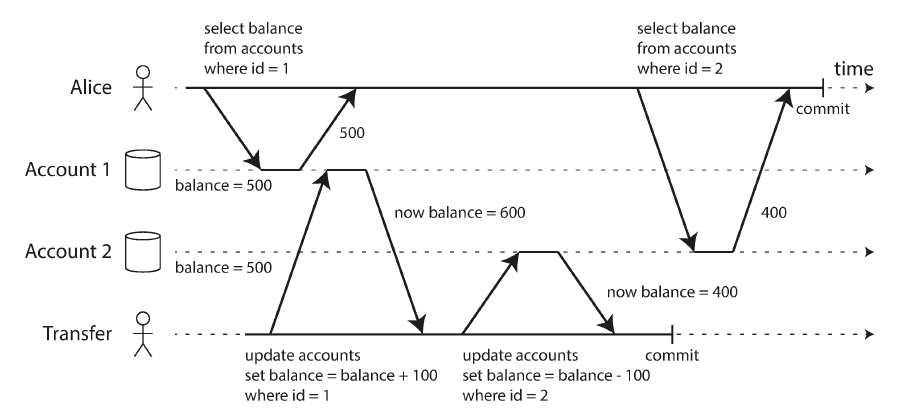
\includegraphics[width=0.5\textwidth]{read-skew.png}
    \caption{Read skew}
\end{figure}

\subsubsection{Repeatable Read or Snapshot Isolation}

\begin{itemize}
    \item Which transaction changes what?
    \begin{itemize}
        \item TODO
    \end{itemize}
    \item "Multi Version Concurrency Control (MVCC)"
    \item Readers do not block writes, writers do not block reads
\end{itemize}

\begin{figure}[H]
    \centering
    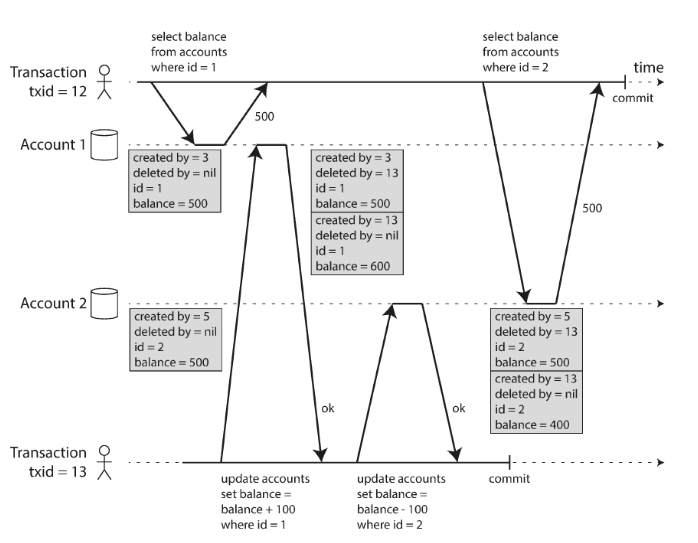
\includegraphics[width=0.5\textwidth]{repeatable-read-of-snapshot-isolation.png}
    \caption{}
\end{figure}

\subsubsection{Multi Version Concurrency Control (MVCC)}

TODO

\subsubsection{Lost updates \& Atomic updates}

\begin{itemize}
    \item Two read - modify - write transactions
    \begin{itemize}
        \item Problem: Bob reads `quantity' while transaction is committing
    \end{itemize}
    \item Solutions: `atomic updates' or manual lock
    \begin{itemize}
        \item No reads or update object until commit
        \item Update `X' SET value = "X2"
        \item (Read - modify - write in one operation)
    \end{itemize}
\end{itemize}

\begin{figure}[H]
    \centering
    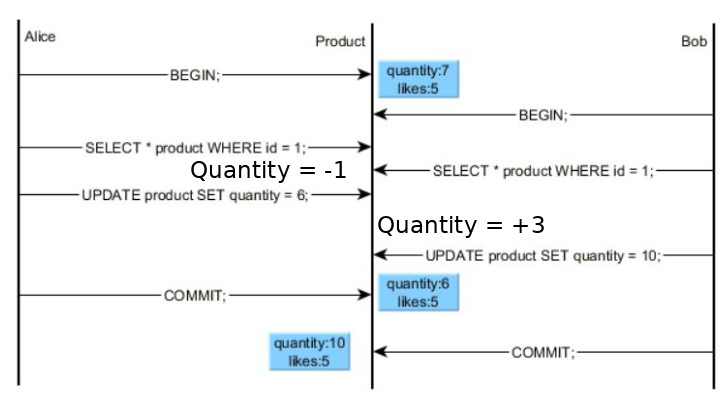
\includegraphics[width=0.5\textwidth]{lost-updates-atomic-updates.png}
    \caption{}
\end{figure}

\subsubsection{Write Skew and others\dots}

\begin{itemize}
    \item Multi object updates \& lost updates
    \item TODO
\end{itemize}

\begin{minted}{sql}
BEGIN TRANSACTION
SELECT COUNT(*) FROM bookings WHERE seat = 'front row'
INSERT INTO bookings ...       -- count > 0
COMMIT;
\end{minted}

\subsubsection{Single Threaded - Serial Execution}

\begin{itemize}
    \item Serial instances for reads
    \begin{itemize}
        \item One fast write thread in RAM
        \item Select on seperate snapshot
    \end{itemize} 
    \item Examples:
    \begin{itemize}
        \item Redis
        \item VoltDB
    \end{itemize} 
    \item Complete transaction in one serial stored procedure
    \begin{itemize}
        \item = piece of code in the DB, already compiled, that is ready to be executed
        \item Upsides: TODO
        \item Downsides: TODO
    \end{itemize}
    \item Partition data
    \begin{itemize}
        \item Multiple threads, one thread per partition
        \item Cross partition transaction? Hard!
    \end{itemize}
\end{itemize}

\subsubsection{2-phase lock - Serial execution}

\begin{itemize}
    \item Weak isolation levels:
    \begin{itemize}
        \item = Readers never block writers, and you can read the old value while it is written
    \end{itemize}
    \item 2PL = exclusive lock on read data, then exclusive lock for writing
    \begin{itemize}
        \item Deadlocks are possible! (= transactions keep waiting for each other's locks)
    \end{itemize}
    \begin{itemize}
        \item Examples:
        \begin{itemize}
            \item MySQL InnoDB
            \item SQL server
            \item DB2 ("Repeatable read")
        \end{itemize}
    \end{itemize}
\end{itemize}

\subsection{Isolation levels}

= Choose between strong isolation or strong performance

\begin{itemize}
    \item Modern processing 8 - 100+ threads
    \item Choose an isolation level:
    \begin{itemize}
        \item Read Uncommitted (weakest isolation, most performance)
        \item Read Committed
        \item Repeatable Read (=snapshot isolation)
        \item Serial Execution (strongest isolation, least performance)
    \end{itemize}
    \item Isolation problems are hard to debug:
    \begin{itemize}
        \item It's a timing problem
        \item Very hard to reproduce
        \item No errors are logged
    \end{itemize}
\end{itemize}

\begin{figure}[H]
    \centering
    \includegraphics[width=0.7\textwidth]{isolation-levels-dbs.png}
    \caption{(default) isolation levels in current databases. (*) Wrong, Oracle does not comply with ANSI}
\end{figure}

\subsubsection{Conclusion}

\begin{itemize}
    \item TODO
\end{itemize}


\subsubsection{Isolation level 1: Read Uncommited}

\begin{itemize}
    \item Read Uncommitted offers no protection agains dirty writes \& dirty reads
    \item Fastest performance, lowest isolation
\end{itemize}


\begin{figure}[H]
    \centering
    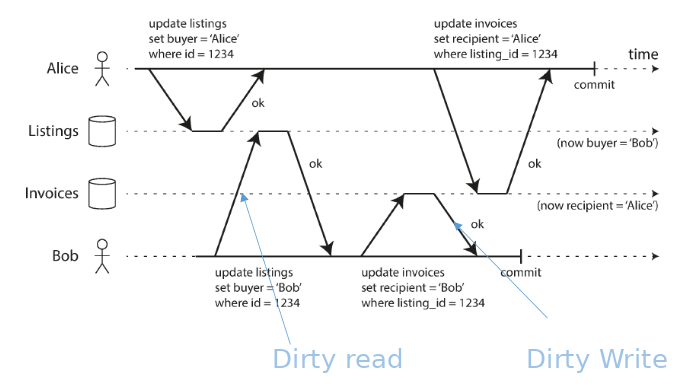
\includegraphics[width=0.5\textwidth]{dirty-reads-lock.png}
    \caption{Dirty read \& dirty write example}
\end{figure}

\subsubsection{Isolation level 2: Read Committed}

\begin{itemize}
    \item No dirty reads
    \item No dirty writes
\end{itemize}

TODO


\textbf{Solutions}

\begin{enumerate}
    \item Read locks (bad performance)
    \item Remember the old value until `commit' (better performance)
\end{enumerate}

\subsection{ACID: Durable}

= A database should be durable: every write transaction has to be written to disk, and should be stored safely and reliably.

\subsubsection{Caching \& BBU}

\begin{itemize}
    \item Write through / back TODO
    \item Battery Backup Unit
    \item RAM caches in SSDs have to be Non-Volatile (NV)!
\end{itemize}

\subsubsection{The transaction chain: innodb\_flush\_log\_at\_try\_commit}



\begin{itemize}
    \item 0: Write the log buffer to the log file and flush the log file \textbf{every second}, but do nothing at transaction commits (fastest)
    \begin{itemize}
        \item Fastest
    \end{itemize}
    \item 1: Write the log buffer to the log file and flush it to durable storage \textbf{at transaction commits}
    \begin{itemize}
        \item This is the only option that is fully ACID compliant
    \end{itemize}
    \item 2: Write the log buffer to the log file \textbf{at every commit}, but flush it every second
\end{itemize}

Flushing = writing to disk

\subsubsection{innodb\_flush\_method}

\begin{itemize}
    \item fdatasync
    \begin{itemize}
        \item InnoDB uses fsync() to flush both data and log files (unix)
    \end{itemize}
    \item O\_DIRECT
    \begin{itemize}
        \item This setting still uses fsync() to flush the files to disk, but it instructs the operating system not to cache the data and not to use read-ahead. Avoids double buffering
    \end{itemize}
    \item async\_unbuffered
    \begin{itemize}
        \item Default value on Windows
        \item Causes InnoDB to use unbuffered I/O for most writes
        \item The exception: it uses buffered I/O to the log files when innodb\_flush\_log\_at\_try\_commit = 2
    \end{itemize}
\end{itemize}

\subsubsection{The Transaction chain}

\begin{figure}[H]
    \centering
    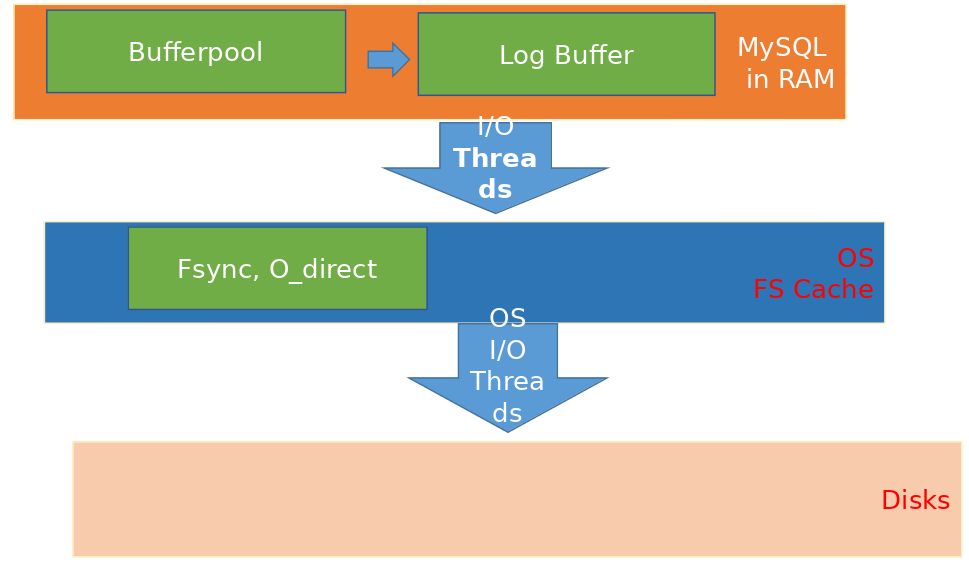
\includegraphics[width=0.5\textwidth]{transaction-chain.png}
    \caption{The transaction chain when writing to disk}
\end{figure}

TODO



\end{document}